% svn info. These are modified by svn at checkout time.
% The last version of these macros found before the maketitle will be the one on the front page,
% so only the main file is tracked.
% Do not edit by hand!
\RCS$Revision: 11362 $
\RCS$HeadURL: svn+ssh://svn.cern.ch/reps/tdr2/notes/AN-11-higgs/trunk/AN-11-higgs.tex $
\RCS$Id: AN-11-higgs.tex 11362 2010-06-25 14:06:15Z alverson $
%%%%%%%%%%%%% ptdr definitions %%%%%%%%%%%%%%%%%%%%%
\input{ptdr-definitions}

%extra-definitions
\newcolumntype{w}[1]{>{\raggedright\hspace{0pt}}p{#1}}
\providecommand{\ttbar}{{$t\bar{t}$}}
\providecommand{\Pythia}{{\textsc{Pythia}}\xspace}
\providecommand{\Tauola}{{\textsc{Tauola}}\xspace}
\providecommand{\Madgraph}{{\textsc{MadGraph}}\xspace}
\providecommand{\Alpgen}{{\textsc{Alpgen}}\xspace}
\providecommand{\Sherpa}{{\textsc{Sherpa}}\xspace}
\providecommand{\MCatNLO}{{\textsc{MCatNLO}}\xspace}
\providecommand{\CMSSW}{{\textsc{CMSSW}}\xspace}
\providecommand{\FastSim}{{\textsc{FastSim}}\xspace}
\providecommand{\FullSim}{{\textsc{FullSim}}\xspace}
\providecommand{\caloMET}{{\textsc{caloMET}}\xspace}
\providecommand{\tcMET}{{\textsc{tcMET}}\xspace}
\providecommand{\pfMET}{{\textsc{pfMET}}\xspace}
\providecommand{\caloJET}{{\textsc{caloJET}}\xspace}
\providecommand{\jpt}{{\textsc{JPT}}\xspace}
\providecommand{\pflow}{{\textsc{pFlow}}\xspace}
\providecommand{\pfJET}{{\textsc{pfJET}}\xspace}
\providecommand{\Roofit}{{\textsc{Roofit}}\xspace}
\providecommand{\TC}{{\textsc{TC}}\xspace}
\providecommand{\TCHE}{{\textsc{TCHE}}\xspace}
\providecommand{\TCHP}{{\textsc{TCHP}}\xspace}
\providecommand{\JP}{{\textsc{JP}}\xspace}
\providecommand{\MET}{{$E_{T}^{miss}$}\xspace}
\providecommand{\RMET}{{${\rm red}\vec{E}_{T}^{miss}$}\xspace}
\providecommand{\MC}{{\textsc{MC}}\xspace}

\linenumbers

%%%%%%%%%%%%%%%  Title page %%%%%%%%%%%%%%%%%%%%%%%%
\cmsNoteHeader{AN-11-higgs} % This is over-written in the CMS environment: useful as preprint no. for export versions
\title{Searching for the Higgs boson\\ in the ZZ$\rightarrow$ 2l2$\nu$ final state\\ with $\sqrt{s}=$7~TeV data}

%Author is always "The CMS Collaboration" for PAS and papers, so author, etc, below will be ignored in those cases

\address[cern]{CERN, Geneva, Switzerland}
%\author[cern]{The CMS Collaboration}
\author[cern]{P.~Silva}
\author[cern]{G.~Cerminara}
\author[cern]{L.~Quertenmont}
\author[cern]{M.~Mannelli}
\author[cern]{M.~Mulders}


% please supply the date in yyyy/mm/dd format. Today has been
% redefined to do so, but it should be fixed as of the final release date.
% For papers and PAS, \today is taken as the date the head file (this one) was last modified according to svn: see the RCS Id string above.
\date{\today}

% Abstract processing:
% 1. **DO NOT use \include or \input** to include the abstract: our abstract extractor will not search through other files than this one.
% 2. **DO NOT use %** to comment out sections of the abstract: the extractor will still grab those lines (and they won't be comments any longer!).
% 3. **DO NOT use tex macros** in the abstract: External TeX parsers used on the abstract don't understand them.
\abstract{
}

% Do not comment out the following hypersetup lines (metadata). They will disappear in NODRAFT mode and are needed by CDS.
% Also: make sure that the values of the metadata items are sensible. For APS submissions, they are automatically converted to APS keywords.
\hypersetup{%
pdfauthor={CMG group},%
pdftitle={Searching for the Higgs in the ZZ to 2 leptons + 2 neutrinos final state with sqrt{s}=7 TeV data},%
pdfsubject={CMS},%
pdfkeywords={CMS, physics, Higgs boson, missing transverse energy}}

\maketitle %maketitle comes after all the front information has been supplied

\begin{small}
\tableofcontents
\end{small}


%
% INTRODUCTION
%
\section{Introduction}
\label{sec:introduction}

%
% EVENT SELECTION
%
\section{Dilepton event selection}
\label{sec:dileptonevselection}

As detailed in the introduction, 
all processes which are expected to produce one or more leptons are considered
to be relevant as concurrent processes with the Higgs dileptonic sample. 
This includes mainly vector boson production (W/Z) and Drell-Yan (DY) processes.
Top quark and di-boson (WW,WZ,ZZ) production are also relevant but with much smaller cross section.
QCD must also be considered for study as jets are expected to fake leptons in the reconstruction process.
Table~\ref{tab:mcsamples} summarizes the simulation samples which are used for all standard model processes
which may mimick the signal under study  .
The global tag GR\_R\_42\_V19 (START42\_V13) has been used to process data (MC) with
version 4\_2\_4 of the CMS official software (CMSSW).
Residual jet energy corrections are applied to data.

\begin{table}[htp]
\caption{List of the SM Monte Carlo samples used in the comparison with 7~TeV data.
For the different processes (signal and background) considered 
the expected cross sections and the corresponding total integrated luminosity are quoted.}
\label{tab:mcsamples}
\begin{center}
\hspace{-1.5cm*}
\begin{tabular}{llll} \hline\hline
\multicolumn{4}{c}{\bf Background processes} \\
Process                      & Dataset                 & $\sigma\cdot BR\cdot k$ (pb) & $L$~(pb$^{-1}$) \\\hline
W+jets                       & /WJetsToLNu\_TuneZ2\_7TeV-madgraph-tauola/S11-S4-v1                    & 31314     & \\
$Z/\gamma^{*}\rightarrow ll$ & /DYJetsToLL\_TuneZ2\_M-50\_7TeV-madgraph-tauola/S11-S4-v1              & 3048      & \\
\ttbar                       & /TTJets\_TuneZ2\_7TeV-madgraph-tauola/S11-S4-v1                        & 165       & \\
\multirow{2}{*}{Single top}  & /T\_TuneZ2\_tW-channel-DR\_7TeV-powheg-tauola/S11-S4-v1 ($t$)          & 7.87      & \\
                             & /Tbar\_TuneZ2\_tW-channel-DR\_7TeV-powheg-tauola/S11-S4-v1 ($\bar{t}$) & 7.87      & \\
\multirow{3}{*}{Dibosons}    & /ZZTo2L2Nu\_TuneZ2\_7TeV\_pythia6\_tauola/S11-v1                       & 0.259     & \\
                             & /WWTo2L2Nu\_TuneZ2\_7TeV\_pythia6\_tauola/S11-v1                       & 4.51      & \\
                             & /WZTo3LNu\_TuneZ2\_7TeV\_pythia6\_tauola/S11-v1                        & 0.596     & \\\hline\hline
\end{tabular}
\end{center}
\end{table}

The next sections summarize the strategy adopted for the trigger, reconstruction and event selection.

%%
%% TRIGGER RECONSTRUCTION EVENT SELECTION
%%
\subsection{Trigger, reconstruction and event selection}
\label{subsec:trigrec}

The main aspects of the event selection are summarized as follows:

\begin{description}

%%% TRIGGER
\item[Trigger] unprescaled double lepton triggers available are used.
Unprescaled single muon triggers are also considered in order to recover possible inefficiencies especially in events with two muons.
Whenever possible, trigger thresholds are chosen below the nominal cut used for the offline reconstruction of electrons and muons.
The following triggers are used: HLT\_Ele17\_CaloIdL\_CaloIsoVL\_Ele8\_CaloIdL\_CaloIsoVL\_v*, HLT\_DoubleMu7\_v*, HLT\_Mu13\_Mu8\_v*,
HLT\_Mu17\_Ele8\_CaloIdL\_v*, HLT\_Mu8\_Ele17\_CaloIdL\_v*, HLT\_IsoMu17\_v*.

%%% PRIMARY VERTICES
\item[Primary vertices] must be found within maximum range of 24~cm along the beam line (z) and within a 2~cm cylinder around the beam line ($\rho$)..
The minimum number of degrees of freedom (n.d.o.f.) of the vertex fit is required to be 4.
In case of multiple primary vertices the primary vertex is chosen to be the one which is highest sum of the transverse momentum of the tracks
and it is required that the selected dileptons' tracks are closer to the chosen vertex by minimizing $\Delta z=z_{PV}-z_{track}^{lepton}$.
It is further required that that $|\Delta z|<$1~cm.

%%% LEPTONS

\item[Leptons] leptons (electrons or muons) are required to be reconstructed with at least $p_T>$5~GeV/c and $|\eta|<$2.5 (2.4) for electrons (muons). 
Electron identification relies on a simple cut based identification algorithm 
which depends on the supercluster shape and its alignment with the track is used for the electrons.
The \texttt{tight} working point of the cut in categories based electron identification is used.
Muon identification is based on the $\chi^2$ fit of the global track and on the number of hits in the tracker and muon stations.
The leptons from signal are expected to be well isolated in the event.
The isolation can be quantified relatively to the transverse momentum of the lepton by
the a particle based isolation $I_{rel}$:

\begin{equation}
I_{rel}=\frac{I_{photons}+I_{neutral~hadrons}+I_{charged~hadrons}}{p_T}
\label{eq:reliso}
\end{equation}

where the sum of photons, neutral hadrons and charged hadrons found in an isolation cone of $\Delta R=$0.3
built around the lepton's momentum are used to compute the correpondent isolations.
As the isolation of the leptons is expected to be affected by pileup events a loose requirement of $I_{rel}<1.0$ is made at this stage of selection.

%%% DILEPTON
\item[Dilepton] for each event with at least 2 leptons selected in the previous conditions all dilepton pair candidates are examined.
The minimum tranvserse momentum of each lepton is required to be $p_T>$20~GeV/c.
The isolation for the leptons is not corrected for pileup/underlying event contributions but it is further tightened.
The deviation introduced in the isolation by the average energy density deposition in the detector ($\rho$) is estimated using the fast jet algorithm.
The details on the algorithm can be found in ~\cite{}.
As the average values for $\rho$, $I_{photons}$ and $I_{neutral~hadrons}$ are expected to increase differently as a function of the number of pileup events
a linear parameterization can be derived for each case. The results of these parameterizations are shown for in Fig~\ref{fig:isolprofile}
for a simulated sample of $Z\rightarrow ll$ events and summarized in Table~\ref{tab:isolprofileparam}.

\FIXME{Needs update}
\begin{figure}[htp]
\begin{center}
%\includegraphics[width=0.49\textwidth]{img/electronIsolationProfile}
%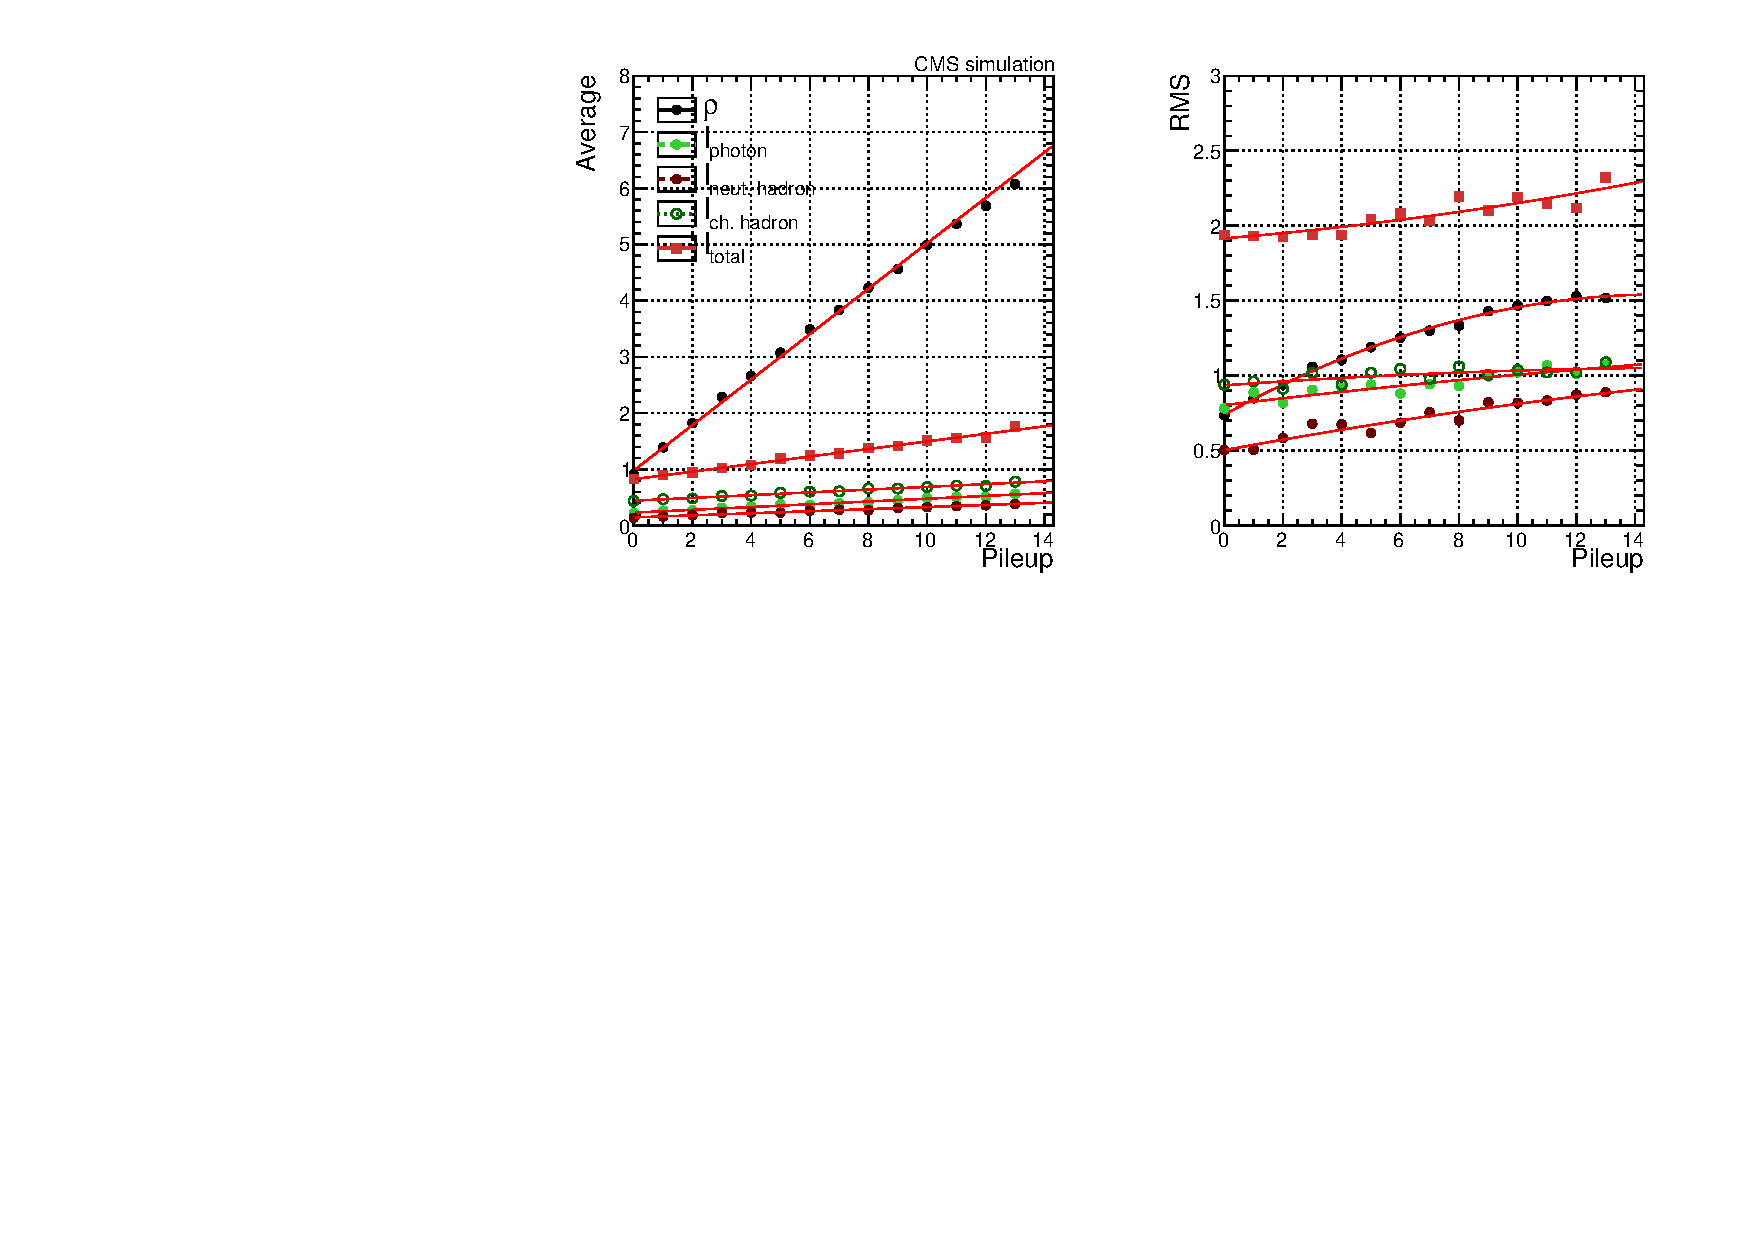
\includegraphics[width=0.49\textwidth]{img/muonIsolationProfile}
\caption{
Isolation and $\rho$ profiles in simulated $Z\rightarrow ll$ events where the leptons have been pre-selected with $I_{rel}<$0.3.
Electrons (muons) are shown on the {\em left} ({\em right}).}
\label{fig:isolprofile}
\end{center}
\end{figure}

\FIXME{Needs update}
\begin{table}[htp]
\caption{Parameterization of pileup dependent quantities, relevant for the isolation of the leptons.
The errors are statistical and result from the fits performed}
\label{tab:isolprofileparam}
\begin{center}
\begin{tabular}{lccc} \hline
Parameter          & Intercept         & Slope             & $\chi^2/dof$ \\ \hline\hline
$\rho$             & 0.586 $\pm$ 0.003 & 0.483 $\pm$ 0.006 & 122/19       \\ \hline
$I_{photons}^{e}$     & 0.604 $\pm$ 0.004 & 0.114 $\pm$ 0.006 & 28/19        \\ 
$I_{neutral hadrons}^{\mu}$   & 0.216 $\pm$ 0.002 & 0.0539 $\pm$ 0.0003 & 13/19      \\ \hline
                   &                   &                     &            \\\hline
$A_{eff}^{e}$      & \multicolumn{3}{c}{0.24 $\pm$ 0.01}                  \\ 
$A_{eff}^{\mu}$    & \multicolumn{3}{c}{0.112 $\pm$ 0.002}                \\ \hline
\end{tabular}
\end{center}
\end{table}

If the event has other isolated leptons, even if failing the minimal $p_T$ requirement, it is rejected.
The dilepton candidate is required to have an invariant mass compatible with a $Z$ boson decay, 
i.e. $|M-M_Z|<$15~GeV/c$^2$ and at least one of the leptons is required to be reconstructed within the 
fiducial region/kinematics of the trigger.

%%% JETS
\item[Jets] jets are selected with $p_T>$15~GeV/c and $|\eta|<5.0$.
Jets are reconstructed with the anti-$k_T$ algorithm with a cone of $R=0.5$. A loose jet id is used based on 
the electromagnetic fraction among other variables.
The simple secondary vertex high efficiency (SSVHE) tagger is used to identify possible $b$-jets.
The medium working point (i.e. SSHVE$>$1.74) is used to tag the jets.  
A veto on events which contain at least one jet tagged by this algorithm is used in order to reduce
the contamination from \ttbar. 

%%% MET
\item[Missing transverse energy] particle flow based \MET is used. The \MET is built from the vectorial sum
of the transverse momentum all particle flow reconstructed candidates.

\end{description}


%%
%% EVENT YIELDS
%%
\subsection{Event yields}
\label{subsec:eventyields}

The event yields after applying the pre-selection discussed in the previous section
are shown in Tables~\ref{tab:presamplecutflow}.

\begin{table}[htp]
\caption{Event yields for a total integrated luminosity of 1091~pb$^{-1}$. The uncertainties quoted are statistical only.}
\label{tab:presamplecutflow}
\begin{center}
\begin{tabular}{lccc} \hline\hline
Process                            & $|M-M_Z|<$15 & 3$^{rd}$-lepton veto & no b-tags\\ \hline
& & & \\\hline
\multicolumn{4}{c}{\bf $\mu\mu$ channel} \\\hline
ZZ                                 & $ 39.17 \pm0.28 $  & $ 39.17 \pm0.28 $  & $ 38.65 \pm0.28 $ \\
WW                                 & $ 67.4 \pm1.6 $  & $ 67.3 \pm1.6 $  & $ 66.6 \pm1.6 $  \\
WZ                                 & $ 73.3 \pm0.7 $  & $ 52.9 \pm0.6 $  & $ 51.5 \pm0.6 $  \\
Single top                         & $ 27.4 \pm0.7 $  & $ 27.1 \pm0.7 $  & $ 11.1 \pm0.4 $  \\
$t\bar{t}$                         & $ 303 \pm5 $  & $ 302 \pm5 $  & $ 66.5 \pm2.3 $  \\
W+jets                             & $ 0.32 \pm0.32 $  & $ 0.32 \pm0.32 $  & $ 0.32 \pm0.32 $ \\
$Z/\gamma^{*}+jets\rightarrow ll$  & $ ( 393.2 \pm0.5 ) \times10^{3} $  & $ ( 392.9 \pm0.5 ) \times10^{3} $  \\
Total expected                     & $ ( 393.7 \pm0.5 ) \times10^{3} $  & $ ( 393.3 \pm0.5 ) \times10^{3} $  & $( 388.3 \pm0.5 ) \times10^{3}$ \\ \hline
data                               & $ 328.5 \times10^{3} $  & $ 328.1 \times10^{3} $  & $  324.1 \times10^{3}$ \\ \hline
& & & \\\hline
\multicolumn{4}{c}{\bf $ee$ channel} \\\hline
ZZ                                 & $ 31.35 \pm0.25 $  & $ 31.32 \pm0.25 $  & $ 30.95 \pm0.25 $  \\
WW                                 & $ 55.4 \pm1.4 $  & $ 55.3 \pm1.4 $  & $ 54.6 \pm1.4 $  \\
WZ                                 & $ 80.6 \pm0.7 $  & $ 44.4 \pm0.5 $  & $ 43.4 \pm0.5 $  \\
Single top                         & $ 24.1 \pm0.6 $  & $ 23.8 \pm0.6 $  & $ 9.9 \pm0.4 $  \\
$t\bar{t}$                         & $ 259 \pm5 $  & $ 257 \pm5 $  & $ 57.8 \pm2.2 $ \\
W+jets                             &  $ 57 \pm8 $  & $ 57 \pm8 $  & $ 55 \pm8 $  \\
$Z/\gamma^{*}+jets\rightarrow ll$  & $ ( 313.1 \pm0.4 ) \times10^{3} $  & $ ( 312.8 \pm0.4 ) \times10^{3} $  & $ ( 308.8 \pm0.4 ) \times10^{3} $ \\
Total expected                     & $ ( 313.6 \pm0.4 ) \times10^{3} $  & $ ( 313.2 \pm0.4 ) \times10^{3} $  & $ ( 309.0 \pm0.4 ) \times10^{3} $ \\\hline
data                               & $ 265.6 \times10^{3} $  & $ 265.2 \times10^{3} $  & $  261.9 \times10^{3} $  \\\hline\hline
\end{tabular}
\end{center}
\end{table}

%%
%%
%%
\section{Verification of the reconstructed missing transverse energy}
\label{sec:met}

%%%
%%% Pileup
%%%
\subsection{Strategies adopted to minimize the effect of pileup}
\label{subsec:pueffects}

\begin{table}[htp]
\caption{}
\label{tab:mettypes}
\begin{center}
\hspace*{-2cm}
\begin{tabular}{llllllll} \hline\hline
\multicolumn{2}{c}{\MET components}                  & PF     & PF no pileup  & track PF              & charged PF & clust. neut. & jet vetoed neut.  \\\hline
\multirow{2}{*}{charged}            & all                      & yes    & -             & -                     & -          & -            & -                    \\
                                    & from PV ($\Delta Z<$cm)  & -      & yes           & yes                   & yes        & yes          & yes                  \\\hline
\multirow{2}{*}{neutrals}           & all                      & yes    & yes           & $p_T>4 \wedge \eta<3$ & no         & no           & yes                  \\
                                    & associated to PV jets    & -      & -             & -                     & -          & yes          & -                    \\
                                    & associated to other jets & -      & -             & -                     & -          & -            & no                   \\\hline\hline
\end{tabular}
\end{center}
\end{table}


%%%
%%% REDUCED MET
%%%
\subsection{Description of the reduced \MET method}
\label{subsec:redmet}

We adopt the definition of reduced missing transverse energy (\RMET) for our analysis.
The definiton is an upgrade of the original concept developed by the D0 collaboration~\cite{Abazov:2008yf}.
The reconstructed \MET is decomposed using either the dilepton direction (in case the two leptons are collimated,
i.e. $\Delta\phi^{ll}<\pi/2$) or the dilepton bisector (in case the two leptons are reconstructed with an open angle,
i.e.   $\Delta\phi^{ll}>\pi/2$).
The bisector of the dilepton is defined transversely to the axis which maximizes the dilepton transverse momentum, 
i.e. the thrust axis($\vec{t}$):

\begin{equation}
\vec{t} =\frac{1}{|\vec{l}_1-\vec{l}_2|}(\vec{l}_1 - \vec{l}_{2})
\label{eq:thrust} 
\end{equation}

where $l_{i}$ is the momentum of the $i$-th lepton. The bisector ($\vec{b}$) is defined in such a way that:

\begin{equation}
\vec{b}\cdot\vec{t}=0 ~~~\wedge~~~ \vec{b}\cdot\vec{l}_1>0
\label{eq:bisector} 
\end{equation}

The thrust and bisector are used to define the projections of the recoil from the jets
(clustered recoil) and the \MET (unclustered recoil) as:

\begin{equation}
R^{\text{clustered}}_{i}=(\sum_{jets} \vec{p}_T) \cdot \hat{i} ~~~~~~~ R^{\text{unclustered}}_{i}=pfMET \cdot \hat{i}
\label{eq:dilrecoilcomponents}
\end{equation}

where $i=t,b$ as defined in Eqs.~\ref{eq:thrust} and ~\ref{eq:bisector}.  
\RMET is defined from the minimum imbalance found using either the clustered or the unclustered recoil of the system.
Each component of \RMET is computed and minimized individually:

\begin{equation}
{\rm red}\cancel{E}_{T_i}^{k} =\vec{p}_{T}^{ll}\cdot \vec{i} + \alpha R^{\text{k}}_{i}
\label{eq:rmet}
\end{equation}

where k=clustered/unclustered. The absolute \RMET measurement is taken from the quadratic sum of the two components.
The procedure just described assumes a conservative scenario for jet energy and unclustered \MET reconstruction and resolution.
It is also expected to be effective against pileup events as jets are seeded using particle flow candidates associated to the
primary vertex selected for each event. Table~\ref{tab:metwp} summarizes the performance of different \MET approaches
regarding the rejection of the Drell-Yan background and the selection of a standard model Higgs with a mass of 200 GeV/$c^{2}$.

\begin{table}[htp]
\caption{Working points for different Drell-Yan rejection powers for standard \MET, projected-\MET and \RMET.}
\label{tab:metwp}
\begin{center}
\begin{tabular}{llll} \hline\hline
\MET                  & PF      & projected  & reduced  \\\hline
                      &        &         & \\
\multicolumn{4}{c}{Medium working point ($10^{-3}$ rejection factor)} \\\hline
Cut value             & 48.4    & 44.1       & 38.9  \\
H(200)                & 49.6\%  & 40.7\%     & 53.2\%  \\\hline
                      &         &             & \\
\multicolumn{4}{c}{Tight working point ($10^{-4}$ rejection factor)} \\\hline
Cut value             & 66.5    & 63.9       & 56.7 \\
H(200)                & 27.5\%  & 20.9\%     & 30.0\% \\\hline\hline
\end{tabular}
\end{center}
\end{table}

%%
%%
%%
\subsection{Data-driven estimation of the instrumental background}
\label{subsec:instrumentalbackground}

Photon candidates are selected from dedicated photon triggered samples.
The samples are summarized in Table~\ref{tab:instrbckgdatasamples}.

\begin{table}[htp]
\begin{center}
\caption{MC and data samples analyzed for the estimation of the instrumental background.
For data the total integrated luminosity and the run range analyzed are shown.
For MC the the cross section and the corresponding integrated luminosity of the analyzed sample are shown.
Z2 is used as a shortname for TuneZ2\_7TeV\_pythia6 and S* for Summer11-PU\_S*\_START42\_V11.
}          
\label{tab:instrbckgdatasamples}
\begin{tabular}{lcl} \hline\hline
\multicolumn{3}{c}{\bf Data} \\
Dataset                               & $L$~(pb$^{-1}$)               & Run range                          \\\hline
/Photon/Run2011A-May10ReReco-v1/AOD   &                               & {\small 160404-163869}             \\
/Photon/Run2011A-PromptReco-v4/AOD    &                               & {\small $>$163869}                 \\
{\bf Total}                           & {\bf }                        &                                    \\\hline
                                      &                               &                                    \\\hline
\multicolumn{3}{c}{\bf MC} \\
Dataset                               & $\sigma$~(pb)                 & $L$~(pb$^{-1}$)                   \\\hline
/G\_Pt-15to30\_Z2/S3-v2/AODSIM        & 1.72$\times$10$^5$            &                                   \\
/G\_Pt-30to50\_Z2/S3-v2/AODSIM        & 1.67$\times$10$^4$            &                                   \\
/G\_Pt-50to80\_Z2/S3-v2/AODSIM        & 2.72$\times$10$^3$            &                                   \\
/G\_Pt-80to120\_Z2/S4-v2/AODSIM       & 4.47$\times$10$^2$            &                                   \\
/G\_Pt-120to170\_Z2/S3-v2/AODSIM      & 84.2                          &                                   \\
/G\_Pt-170to300\_Z2/S4-v2/AODSIM      & 22.6                          &                                   \\
/G\_Pt-300to470\_Z2/S3-v2/AODSIM      & 1.49                          &                                   \\
/G\_Pt-470to800\_Z2/S3-v2/AODSIM      & 0.132                         &                                   \\
/G\_Pt-800to1400\_Z2/S3-v2/AODSIM     & 3.48$\times$10$^{-3}$         &                                   \\
/G\_Pt-1400to1800\_Z2/S3-v2/AODSIM    & 1.26$\times$10$^{-5}$         &                                   \\\hline\hline
\end{tabular}
\end{center}
\end{table}

For each triggered event the highest $p_T$ photon trigger candidate is chosen.
The offline reconstructed photon is required to have a $E_T$ 
greater than that of the trigger threshold it fired.
Further identification and isolation requirements are made as summarized in Table~\ref{tab:photonsel}
and are based on~\cite{Khachatryan:2010fm}.

\begin{table}[htp]
\begin{center}
\caption{Photon selection requirements according to the region of reconstruction in the electromagnetic calorimeter.}
\label{tab:photonsel}
\begin{tabular}{lcc} \hline\hline
Variable                              & ECAL barrel                        & ECAL endcap                   \\\hline
$E_T$                                 & \multicolumn{2}{c}{trigger dependent}                              \\
$|\eta|$                              & $<$1.4442                          & 1.566$<|\eta|<$2.5            \\ 
$\sigma_{i\eta i\eta}$                & 0$<\sigma<$0.013                   & 0$<\sigma<$0.03               \\ 
$\sigma_{i\phi i\phi}$                & $>$0                               & -                             \\ 
seed rec. hit flag                    & $\neq$ kOutOfTime                  & -                             \\ 
$h/e$                                 & $<$0.05                            & $<$0.5                        \\ 
Tracker isolation                     & \multicolumn{2}{c}{$<$2.0 + 0.001$E_T$}                            \\ 
ECAL isolation                        & \multicolumn{2}{c}{$<$4.2 + 0.003$E_T$}                            \\ 
HCAL isolation                        & \multicolumn{2}{c}{$<$2.2 + 0.001$E_T$}                            \\\hline 
\end{tabular}
\end{center}
\end{table}

%
%
%
\section{Search for the standard model Higgs in the 2l2$\nu$ final state}
\label{sec:higgssearch}


%%
%% Higgs event selection
%%
\subsection{Higgs event selection}
\label{subsec:higgsselection}


%%
%% Discriminator analysis
%%
\subsection{Discriminator based analysis of the selected events}
\label{subsec:discanalysis}

%%
%% Background determination
%%
\subsection{Background determination}
\label{subsec:backgrounddet}

%%
%%
%%
\subsection{Efficiency of the selection}
\label{subsec:selefficiency}

%%
%%
%%
\subsection{Systematic uncertainties}
\label{subsec:systunc}


%
%
%
\section{Exclusion limits}
\label{sec:excllimits}


%
% CONCLUSIONS
%
\section{Conclusions}
\label{sec:conclusions}




%% **DO NOT REMOVE BIBLIOGRAPHY**
\bibliography{auto_generated}   % will be created by the tdr script.

  
\end{document}


